

\begin{exercise}{Clipping - 4 Pkt.}
\label{ex-de-mt-clipping-002}
Erkl�ren sie den Prozess des Clippings. \\
Gegeben sei folgende Szene, angegeben als Menge primitiver Objekte im SVG Koordinatensystem:  
\begin{itemize}
  \item $G_1=(1,2,12,15)$
  \item $G_2=(6,6,8,9)$
  \item $G_3=(2,12,15,1)$
  \item $R_1=(1,2,13,11)$
  \item $R_2=(4,6,9,2)$
\end{itemize}
Zeichnen sie die Szene im Weltkoordinatensystem und f�hren sie danach ein 
Clipping f�r das Rechteck $(5,5,5,5)$ unter Verwendung des Linien-Clipping Algorithmus von Cohen und Sutherland durch. 
\\

Bemerkung: Rechtecke sind in der Form $R=(x_0,y_0,Breite,H\"ohe)$ gegeben und Geraden als $G=(x_0,y_0,x_1,y_1)$. 

\answer{
Gezeichnete Szene:\\

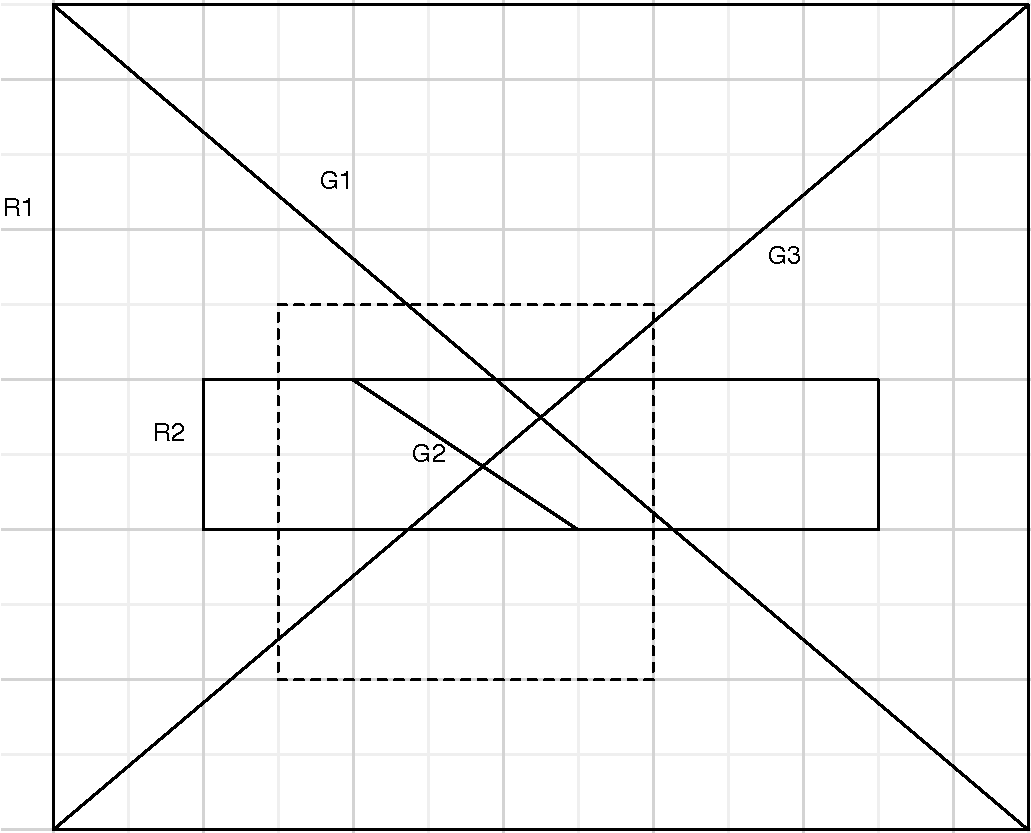
\includegraphics[width=0.5\textwidth]{figure/clipping-ohne}

Clipping Bitbelegung:\\
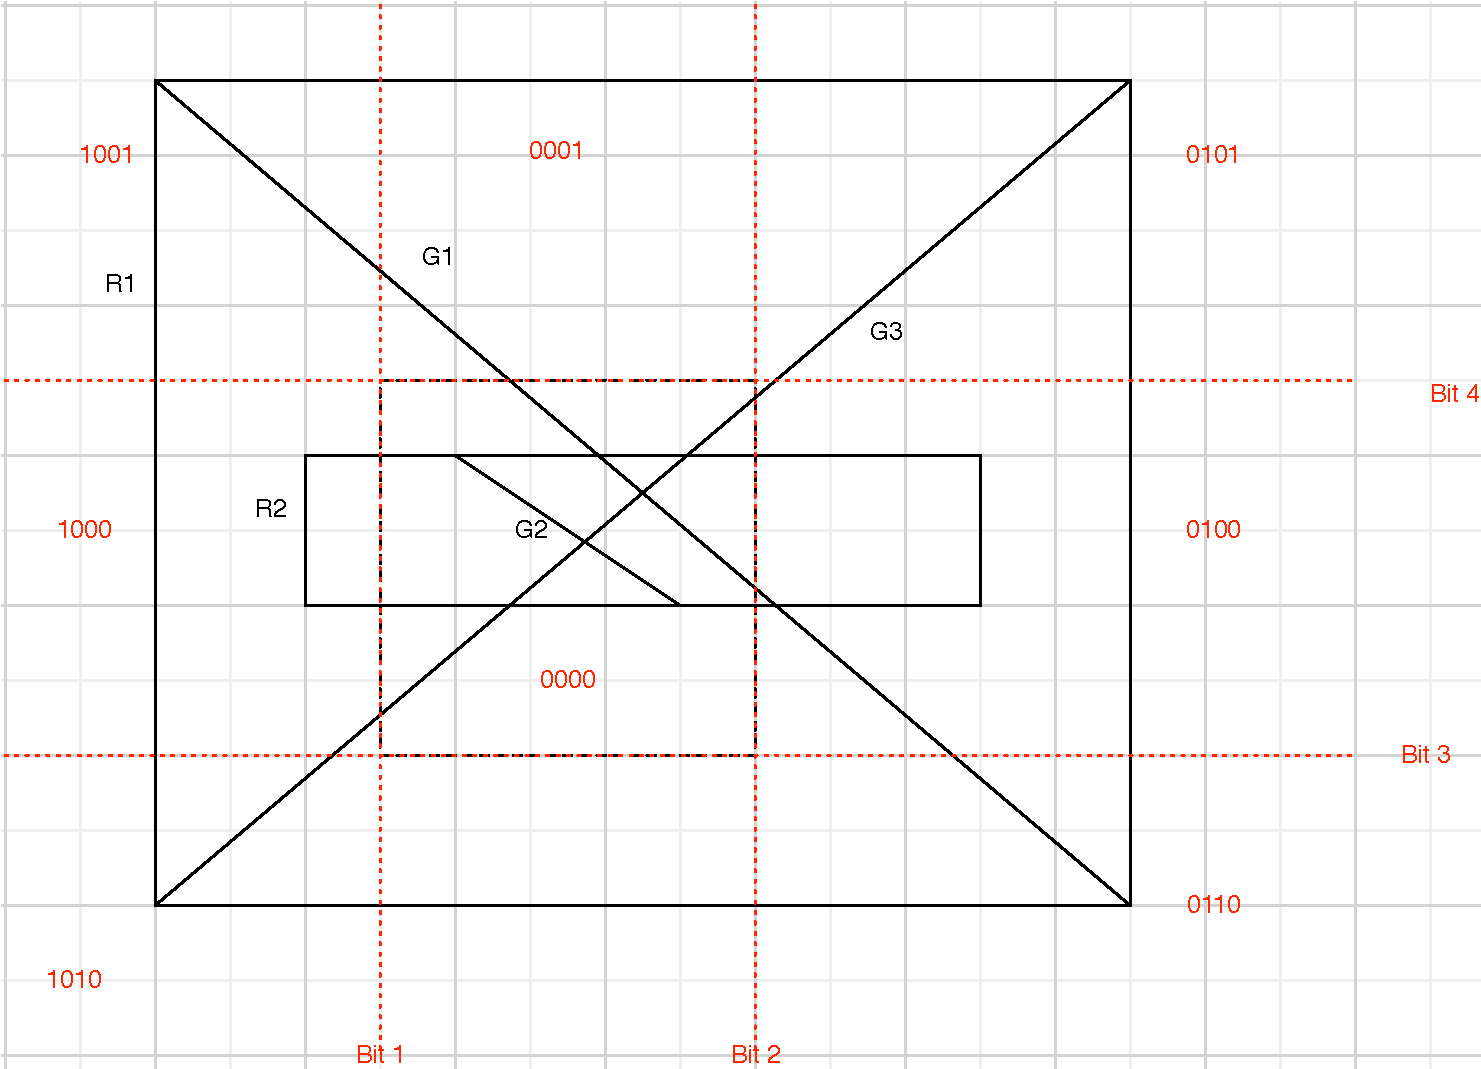
\includegraphics[width=0.5\textwidth]{figure/clipping-mit}

Wenn Linien $P_1\;OR\;P_2=0000$, dann ist diese im Clipping Fenster\\
 
Wenn Linien $P_1\;AND\;P_2\neq 0000$, dann ist diese Linie in den Randbereichen und nicht zu zeichnen.\\

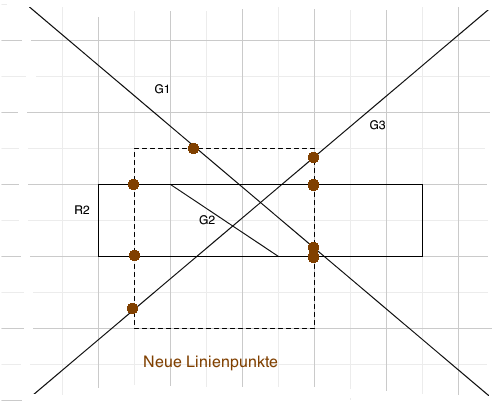
\includegraphics[width=0.5\textwidth]{figure/clipping-final}

}


\end{exercise}

